\documentclass[12pt,a4paper]{article}

\usepackage[utf8]{inputenc}
\usepackage[T1]{fontenc}
\usepackage[brazil]{babel}
\usepackage{geometry}
\usepackage{graphicx}
\usepackage{booktabs}
\usepackage{float}
\usepackage{amsmath}
\usepackage{hyperref}
\usepackage{caption}
\usepackage{setspace}

\geometry{margin=2.5cm}
\onehalfspacing
\hypersetup{colorlinks=true, linkcolor=black, urlcolor=blue, citecolor=black}

\title{Comparação de classificadores ImageNet em vídeo gravado e webcam}
\author{João \and Wesley \and André}
\date{Outubro de 2026}

\begin{document}
\maketitle

\begin{abstract}
Este relatório descreve a etapa de classificação de um pipeline de visão computacional.
Três modelos pré-treinados no ImageNet --- ResNet-50, EfficientNet-B0 e ViT-B/16 ---
foram comparados em um vídeo gravado e em uma webcam. No vídeo, cada modelo processou
330 quadros. A avaliação quantitativa usou 50 quadros anotados com as classes
\texttt{backpack}, \texttt{water bottle} e \texttt{computer keyboard}.
ResNet-50 e ViT-B/16 alcançaram 56\% de acurácia top-1; o EfficientNet-B0 alcançou 26\%,
mas foi o mais rápido, com 25,5 quadros por segundo na inferência em CPU.
A acurácia top-5 ficou entre 74\% e 88\%, indicando que a classe correta frequentemente
permanece entre as alternativas, mesmo quando não é a primeira.
Todos os experimentos de tempo foram executados em CPU, pois a GPU não estava disponível.
\end{abstract}

\section{Introdução}

Classificar o conteúdo de um quadro é a primeira decisão de muitos sistemas de visão:
antes de localizar, rastrear ou segmentar um objeto, o modelo precisa atribuir uma
categoria à imagem. Redes treinadas no ImageNet já oferecem essa capacidade sem exigir
um novo treinamento, o que permite comparar arquiteturas diferentes sob o mesmo vocabulário
de mil classes.

O objetivo deste trabalho é comparar três famílias de classificadores:
uma rede residual convolucional, uma rede convolucional compacta obtida por busca e
escala composta, e um transformador visual. A comparação considera tanto a qualidade
da classificação quanto o custo computacional, em dois cenários:
\begin{enumerate}
    \item vídeo gravado, com anotação de referência em quadros espaçados;
    \item webcam, com medição de latência e taxa de quadros em tempo real.
\end{enumerate}

A cena escolhida contém uma mochila, uma garrafa vermelha e um teclado sobre uma
superfície clara. Esses objetos pertencem ao vocabulário do ImageNet e aparecem com
variações de distância, ângulo, corte e presença simultânea.

\section{Fundamentação teórica}

\subsection{Classificação de imagens}

Um classificador recebe uma imagem \(x\) e produz uma distribuição
\(p(y \mid x)\) sobre um conjunto fechado de classes. A decisão top-1 é a classe de
maior probabilidade. A decisão top-\(k\) é considerada correta quando a classe de
referência está entre as \(k\) maiores probabilidades. Neste trabalho, \(k = 5\) no
vídeo e \(k = 3\) na exibição da webcam.

O ImageNet-1K reúne cerca de 1,2 milhão de imagens de treinamento distribuídas em mil
categorias \cite{russakovsky2015}. Os nomes usados como referência precisam coincidir
exatamente com essa lista. Classes visualmente próximas, como \texttt{computer keyboard}
e \texttt{space bar}, ou \texttt{backpack} e \texttt{mailbag}, competem entre si mesmo
quando um observador humano considera a resposta evidente.

\subsection{Redes convolucionais e ResNet-50}

Uma rede convolucional aplica filtros locais que detectam bordas, texturas e, nas
camadas mais profundas, partes de objetos. O empilhamento dessas camadas aumenta a
capacidade de representação, mas redes muito profundas podem sofrer degradação do
treinamento: acrescentar camadas deixa de melhorar, e pode piorar, a solução encontrada.

A ResNet introduz conexões residuais \cite{he2016}. Em vez de aprender diretamente um
mapeamento \(H(x)\), um bloco aprende um resíduo \(F(x)\) e devolve
\[
    y = F(x) + x.
\]
A identidade \(x\) continua disponível para as camadas seguintes. Isso facilita a
propagação do gradiente e permite treinar redes com dezenas ou centenas de camadas.
A ResNet-50 usada aqui possui 50 camadas ponderadas, gargalos com convoluções
\(1 \times 1\), \(3 \times 3\) e \(1 \times 1\), e 25,6 milhões de parâmetros.
Os pesos são \texttt{IMAGENET1K\_V2}, acompanhados da transformação oficial de
redimensionamento, recorte central e normalização.

\subsection{EfficientNet-B0}

Aumentar uma rede convolucional pode significar torná-la mais profunda, mais larga ou
capaz de receber imagens maiores. Fazer apenas uma dessas mudanças costuma desperdiçar
capacidade. A família EfficientNet equilibra as três dimensões por meio de um coeficiente
composto \cite{tan2019}. A variante B0 é o modelo-base: pequena, com convoluções
profundamente separáveis e blocos do tipo \emph{inverted bottleneck}, inspirados nas
redes móveis.

O EfficientNet-B0 deste experimento tem 5,3 milhões de parâmetros, cerca de um quinto
da ResNet-50, e usa os pesos \texttt{IMAGENET1K\_V1}. A expectativa teórica é obter
boa eficiência, com alguma perda de capacidade diante de objetos pequenos ou ambíguos.

\subsection{Vision Transformer}

O ViT divide a imagem em fragmentos quadrados, trata cada fragmento como um token e
processa a sequência com atenção \cite{dosovitskiy2021}. Na variante B/16, cada
fragmento tem \(16 \times 16\) pixels e o codificador segue a escala Base, com
86,6 milhões de parâmetros. Diferentemente da convolução, a atenção pode relacionar
regiões distantes desde as primeiras camadas. O custo cresce com o número de tokens,
o que torna essa arquitetura mais pesada em CPU.

O modelo foi carregado com os pesos \texttt{IMAGENET1K\_V1} e com a transformação
associada a esses pesos. Assim, cada rede recebe a imagem no tamanho e na normalização
para os quais foi treinada.

\subsection{Métricas de qualidade e de eficiência}

A acurácia top-1 mede a fração de quadros em que a primeira classe coincide com o
rótulo. A acurácia top-5 aplica o mesmo critério às cinco primeiras classes.
Precisão, revocação e F1 são calculadas na média macro: cada classe observada recebe
o mesmo peso, independentemente de sua frequência. Essa escolha é rigorosa quando o
modelo inventa muitas classes erradas, pois cada classe espúria reduz a média.

A latência é o tempo da inferência, em milissegundos, depois de dez execuções de
aquecimento. O FPS de inferência é \(1000\) dividido pela latência média e não inclui
a leitura ou a gravação do vídeo. Na webcam, o FPS exibido usa uma média móvel do
ciclo completo, enquanto o resumo também registra a latência média e o percentil 95.

\section{Materiais e método}

\subsection{Vídeo e anotação}

O vídeo tem resolução \(464 \times 832\), duração de 28,7 segundos, 1.648 quadros e
taxa média de 57,4 quadros por segundo. O processamento classificou um quadro a cada
cinco, totalizando 330 inferências por modelo. Todos os quadros foram preservados nos
vídeos de saída, repetindo a última classificação disponível nos quadros intermediários.

Cinquenta quadros, espaçados de modo uniforme entre os quadros processados, receberam
um rótulo de referência. Como vários objetos podem aparecer juntos, o rótulo indica o
objeto principal ou mais central. A distribuição ficou em 25 mochilas, 13 teclados e
12 garrafas. Os nomes gravados foram exatamente \texttt{backpack},
\texttt{computer keyboard} e \texttt{water bottle}.

\subsection{Execução}

Os modelos foram obtidos pelo \texttt{torchvision}, em modo de avaliação, com seleção
automática entre CUDA e CPU. Nesta máquina, a execução ocorreu em CPU. Cada modelo
recebeu dez inferências de aquecimento antes da medição. O código prevê
\texttt{torch.cuda.synchronize()} quando há GPU; como não havia CUDA, o pico de memória
da GPU permaneceu indisponível.

A webcam foi executada no Windows, porque o subsistema Linux não expõe a câmera.
A câmera 0 forneceu quadros de \(640 \times 480\). Durante o teste, as teclas 1, 2 e 3
alternaram ResNet-50, EfficientNet-B0 e ViT-B/16, e a tecla \texttt{q} encerrou a sessão.

\section{Resultados no vídeo}

A Tabela~\ref{tab:comparacao} resume qualidade e custo. ResNet-50 e ViT-B/16 empatam
em acurácia top-1, mas a ResNet é cerca de 2,4 vezes mais rápida e possui menos de
um terço dos parâmetros do ViT. O EfficientNet-B0 é o menor e o mais rápido, embora
sua acurácia top-1 seja menos da metade da observada nos outros dois.

\begin{table}[H]
\centering
\caption{Comparação no vídeo gravado, em CPU, sobre 50 quadros anotados.}
\label{tab:comparacao}
\begin{tabular}{lrrrrr}
\toprule
Modelo & Parâmetros & Top-1 & Top-5 & Latência & FPS \\
\midrule
ResNet-50 & 25,6 mi & 56\% & 88\% & 114,3 ms & 8,75 \\
EfficientNet-B0 & 5,3 mi & 26\% & 74\% & 39,2 ms & 25,52 \\
ViT-B/16 & 86,6 mi & 56\% & 82\% & 278,3 ms & 3,59 \\
\bottomrule
\end{tabular}
\end{table}

A precisão, a revocação e a F1 macro foram baixas: 0,210 para a ResNet-50, 0,071 para
o EfficientNet-B0 e 0,182 para o ViT-B/16. Esses valores não contradizem a acurácia
top-1. A média macro percorre também as classes erradas produzidas pelos modelos,
como \texttt{space bar}, \texttt{mailbag}, \texttt{joystick} e \texttt{safe}.
Uma única ocorrência de uma classe estranha recebe o mesmo peso de uma classe verdadeira
frequente. Por isso, a acurácia top-1 e a top-5 descrevem melhor o desempenho nesta
amostra, enquanto a F1 macro evidencia a dispersão dos erros.

\begin{figure}[H]
    \centering
    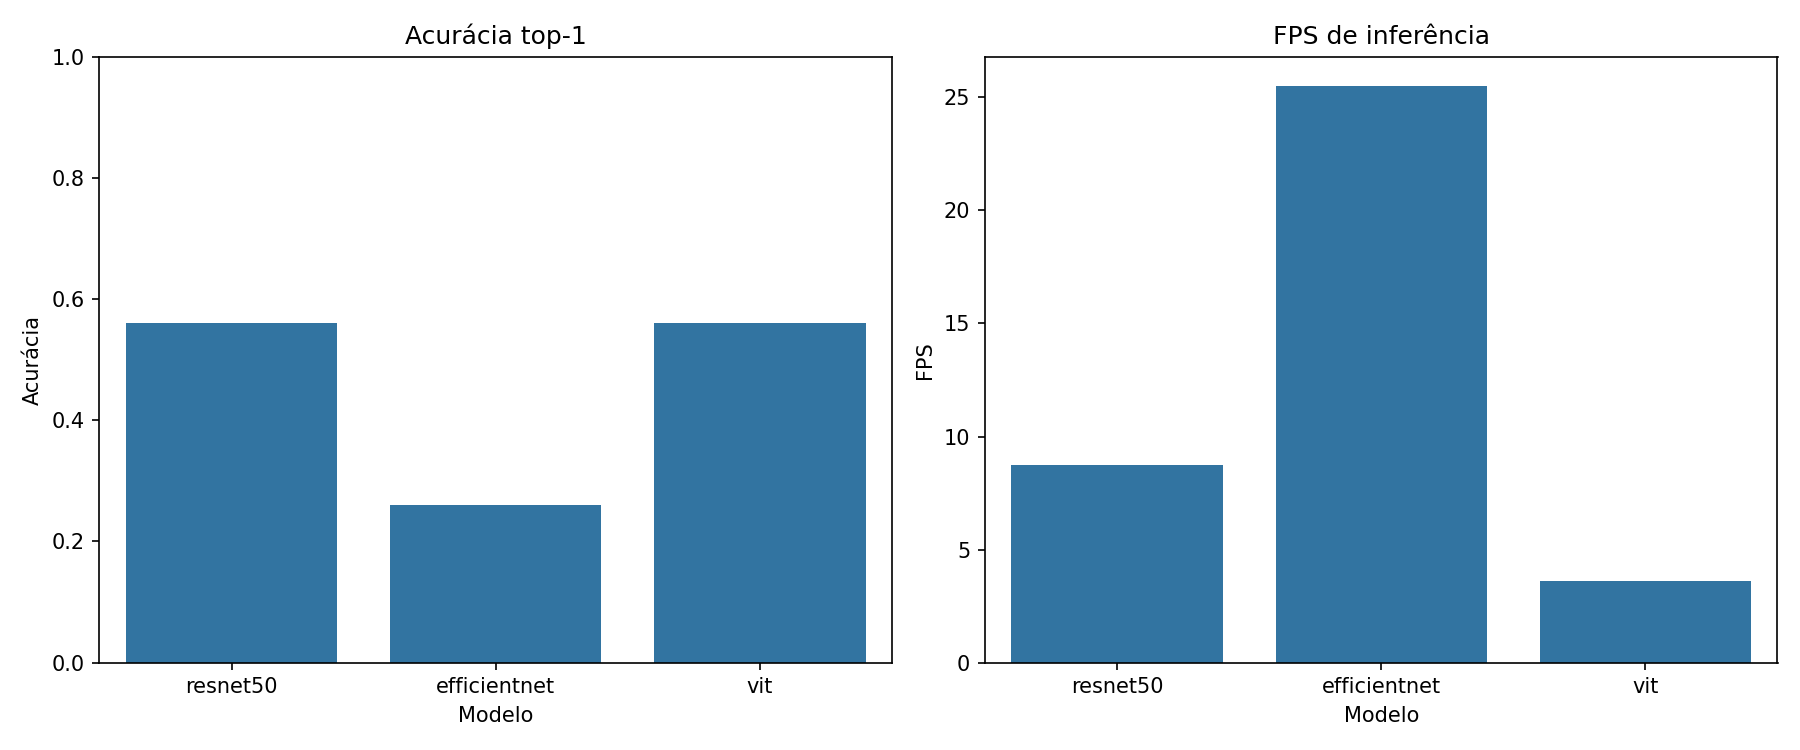
\includegraphics[width=\textwidth]{imagens/accuracy_vs_fps.png}
    \caption{Acurácia top-1 e FPS de inferência no vídeo.}
    \label{fig:barras}
\end{figure}

\begin{figure}[H]
    \centering
    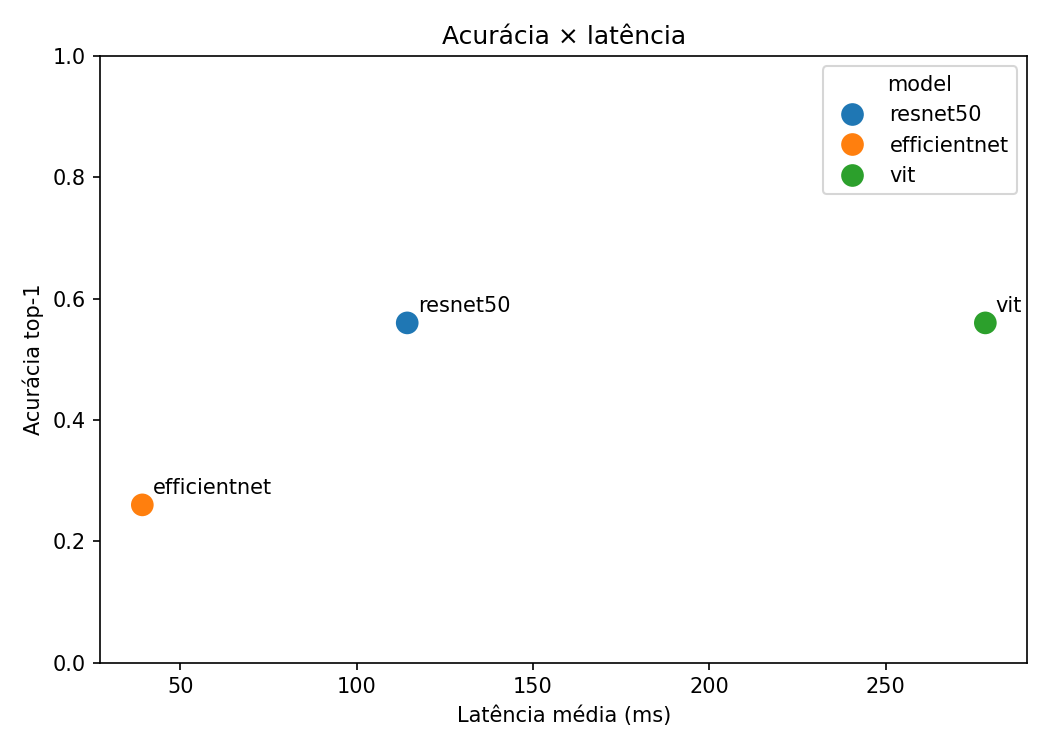
\includegraphics[width=0.78\textwidth]{imagens/accuracy_vs_latency.png}
    \caption{Relação entre acurácia top-1 e latência média.}
    \label{fig:dispersao}
\end{figure}

\subsection{Desempenho por classe}

A Tabela~\ref{tab:classes} mostra que a mochila é a classe mais estável. O teclado é
o principal ponto de falha: ResNet-50 e EfficientNet-B0 não acertaram nenhuma decisão
top-1, embora a ResNet ainda colocasse o teclado entre as cinco primeiras classes em
69\% desses quadros. O ViT foi o único a acertar o teclado no top-1, em 38\% dos casos,
e também obteve a melhor taxa para a garrafa.

\begin{table}[H]
\centering
\caption{Acurácia por classe de referência.}
\label{tab:classes}
\begin{tabular}{lrrr}
\toprule
Classe & ResNet-50 & EfficientNet-B0 & ViT-B/16 \\
\midrule
Mochila (25) & 88\% / 100\% & 44\% / 92\% & 60\% / 100\% \\
Teclado (13) & 0\% / 69\% & 0\% / 46\% & 38\% / 54\% \\
Garrafa (12) & 50\% / 83\% & 17\% / 67\% & 67\% / 75\% \\
\bottomrule
\end{tabular}
\end{table}

\noindent Cada célula apresenta acurácia top-1 seguida da acurácia top-5.

\subsection{Erros qualitativos}

Foram registrados 22 erros da ResNet-50, 37 do EfficientNet-B0 e 22 do ViT-B/16.
Os padrões se repetem e podem ser associados à aparência da cena:

\begin{itemize}
    \item \textbf{Objeto pequeno ou excêntrico.} Quando o teclado ocupa uma faixa
    estreita à direita, a ResNet frequentemente responde \texttt{space bar}. A tecla
    de espaço faz parte do próprio objeto, mas não é a categoria desejada.
    \item \textbf{Classes visualmente vizinhas.} A mochila foi confundida com
    \texttt{mailbag}. A troca é compreensível: ambas são bolsas escuras e flexíveis.
    O ViT manteve \texttt{backpack} no top-5 em todos os quadros de mochila.
    \item \textbf{Vários objetos no quadro.} A garrafa vermelha compete com a mochila
    dominante. O ViT chegou a atribuir mais de 80\% de confiança à garrafa em quadros
    cuja referência era a mochila, porque a garrafa permanecia nítida na borda.
    \item \textbf{Confusão geométrica.} O EfficientNet-B0 trocou a mochila por
    \texttt{bulletproof vest} ou \texttt{joystick}. A superfície escura e retangular,
    vista de perto, perde as alças e o contorno característicos da mochila.
    \item \textbf{Baixa confiança e classe implausível.} Em quadros superiores e
    parcialmente cortados, os três modelos produziram \texttt{safe} com confiança
    variável. O ViT chegou a 96\% em um quadro no qual a garrafa era o objeto central.
    Esse caso mostra que alta confiança não garante correção.
\end{itemize}

As matrizes de confusão estão em
\texttt{imagens/confusion\_matrix\_resnet50.png},
\texttt{imagens/confusion\_matrix\_efficientnet.png} e
\texttt{imagens/confusion\_matrix\_vit.png}. As listas quadro a quadro estão em
\texttt{outputs/errors\_<modelo>.csv}.

\section{Resultados na webcam}

A Tabela~\ref{tab:webcam} confirma a mesma ordem de eficiência. O EfficientNet-B0
manteve cerca de 15 FPS no ciclo medido, com latência p95 de 50,8 ms. A ResNet-50
permaneceu perto de 6 FPS, e o ViT-B/16 perto de 2,8 FPS, com p95 de 342 ms.
A alternância pelas teclas funcionou sem reiniciar o programa: cada modelo foi
carregado e aquecido apenas na primeira seleção.

\begin{table}[H]
\centering
\caption{Resumo da sessão de webcam em CPU.}
\label{tab:webcam}
\begin{tabular}{lrrrr}
\toprule
Modelo & Quadros & FPS médio & Latência média & Latência p95 \\
\midrule
ResNet-50 & 159 & 6,09 & 124,5 ms & 167,8 ms \\
EfficientNet-B0 & 410 & 15,17 & 42,2 ms & 50,8 ms \\
ViT-B/16 & 133 & 2,78 & 280,7 ms & 342,1 ms \\
\bottomrule
\end{tabular}
\end{table}

A webcam não possui rótulos de referência, portanto esses números medem apenas
responsividade. O FPS da webcam é menor do que o FPS de inferência do vídeo porque
inclui captura, desenho e exibição. As predições observadas na cena da sala foram
instáveis e, em geral, pouco específicas, o que é esperado: pessoas, roupas e
ambientes internos não formam um único objeto central das mil classes.

\section{Discussão}

Não há um vencedor único. A escolha depende da restrição principal:
\begin{itemize}
    \item a ResNet-50 oferece o melhor equilíbrio nesta amostra, com a maior acurácia
    top-5, bom reconhecimento da mochila e custo intermediário;
    \item o ViT-B/16 acompanha a acurácia top-1 e reconhece melhor teclado e garrafa,
    mas o tempo por quadro limita o uso interativo em CPU;
    \item o EfficientNet-B0 é adequado quando a taxa de quadros é a prioridade e uma
    revisão posterior, humana ou por outro modelo, pode recuperar erros.
\end{itemize}

O pré-treinamento no ImageNet explica tanto os acertos quanto as confusões. Os modelos
não foram ajustados à mesa, à iluminação ou à câmera deste vídeo. Eles respondem com a
categoria global mais semelhante, mesmo que a imagem contenha três objetos. Uma etapa
posterior de detecção seria mais adequada para contar e localizar cada item.

As limitações são o tamanho da anotação, a existência de um único vídeo, a regra de um
rótulo por quadro e a ausência de GPU. Cinquenta quadros bastam para observar tendências,
mas não para estimar diferenças pequenas entre modelos. A F1 macro deve ser lida junto
com a lista de classes preditas, pois a dispersão dos erros influencia fortemente essa média.

\section{Conclusão}

A etapa de classificação comparou ResNet-50, EfficientNet-B0 e ViT-B/16 com suas
transformações oficiais e com o vocabulário do ImageNet. No vídeo anotado, ResNet-50 e
ViT-B/16 alcançaram 56\% de acurácia top-1, enquanto o EfficientNet-B0 alcançou 26\%.
A ResNet-50 reuniu a melhor acurácia top-5, 88\%, e uma latência intermediária de
114 ms. O EfficientNet-B0 foi aproximadamente três vezes mais rápido que a ResNet e
sete vezes mais rápido que o ViT.

Os erros concentram-se no teclado, em objetos cortados e em quadros com mais de um
objeto. Alta confiança não eliminou trocas graves, como a classificação de uma garrafa
como cofre. A webcam reproduziu a ordenação de velocidade e demonstrou a troca de
modelo durante a execução.

\begin{thebibliography}{9}

\bibitem{he2016}
K. He, X. Zhang, S. Ren e J. Sun.
\newblock Deep Residual Learning for Image Recognition.
\newblock \emph{IEEE Conference on Computer Vision and Pattern Recognition}, 2016.

\bibitem{tan2019}
M. Tan e Q. V. Le.
\newblock EfficientNet: Rethinking Model Scaling for Convolutional Neural Networks.
\newblock \emph{International Conference on Machine Learning}, 2019.

\bibitem{dosovitskiy2021}
A. Dosovitskiy et al.
\newblock An Image is Worth 16x16 Words: Transformers for Image Recognition at Scale.
\newblock \emph{International Conference on Learning Representations}, 2021.

\bibitem{russakovsky2015}
O. Russakovsky et al.
\newblock ImageNet Large Scale Visual Recognition Challenge.
\newblock \emph{International Journal of Computer Vision}, 2015.

\end{thebibliography}

\end{document}
